\documentclass[10pt,pdf,hyperref={unicode}]{beamer}

\usepackage[T2A]{fontenc}
\usepackage{amssymb,amsmath}
\usepackage[english,russian]{babel}
\usepackage{setspace} %TO DO!!!	
\usepackage{graphicx}
\usepackage{graphics} % for pdf, bitmapped graphics files
\usepackage{epstopdf}
\usepackage{epsfig}
\usepackage{subfig}
\usepackage{epsf}
\usepackage{movie15}
\usepackage{hyperref}
\usepackage{beamerthemesplit}
\usepackage{float}
\usepackage{wrapfig}

\usepackage{amssymb,amsfonts,amsmath,mathtext}
\usepackage{cite,enumerate,float,indentfirst}

\graphicspath{{fig/}}
\usetheme[numbers, totalnumbers, compress, mylogo]{Statmod}
\setbeamercovered{transparent}
\setbeamertemplate{navigation symbols}{}

\title[]{Output Robust Control with Anti-Windup Compensation for Robotic Boat }

\author[]{\textbf{Igor~V.~Petranevsky}, Oleg~I.~Borisov, Vladislav~S.~Gromov, Anton~A.~Pyrkin, , Alexey~A.~Bobtsov, Alexey~O.~Klyunin}

\institute{\small
ITMO University, St. Petersburg, Russia\\
Institute for Problems of Mechanical Engineering, St. Petersburg, Russia\\
\vspace{5mm}
21st International Conference on Methods and Models in Automation and Robotics}

\date{August 29 - September 1, 2016\\
Miedzyzdroje, Poland}

\begin{document}

\begin{frame}

\maketitle

\end{frame}

%============================================================================================

\begin{frame}{Outline}

\begin{center}
\tableofcontents
\end{center}

\end{frame}

%============================================================================================

\section{Overview}

\begin{frame}{Introduction}

\begin{center}
{\Large Prerequisite\\
\vspace{0.5cm}
\textbf{Why output control?}}
\end{center}

\vspace{0.5cm}

Output control approaches are significantly useful, when measurements of output derivatives are complicated or even impossible due to different reasons.

\vspace{0.3cm}

Design of robust regulator is important for engineers because
\begin{itemize}
	\item precise parameters of plants may be unknown or they can be changed during operations
	\item all real technical systems are actually constrained 
	
\end{itemize}

\end{frame}

\begin{frame}{Introduction}
	
\begin{center}
{\Large Choosing method\\
	\vspace{0.5cm}
	\textbf{Why consecutive compensator?}}
\end{center}

\vspace{0.3cm}

It was proved and applied 
\begin{itemize}
	\item for linear plants
	\item for nonlinear plants
	\item for tracking problem with compensation of external disturbances
	\item  for time-delay systems 
\end{itemize}

\vspace{0.3cm}

The main advantage of this approach is simplicity of engineering implementation in the cases of plant uncertainties and unavailability of output derivatives.

\end{frame}

\begin{frame}{Introduction}
	
	\begin{center}
		{\Large \textbf {Input saturation}\\}
	\end{center}
	
	\vspace{0.3cm}
	
	Anti-windup is frequently used approach in wide range of applications to solve the problem of input saturation - one of the significant problems related with implementation of theoretical results in real systems
	
	\vspace{0.3cm}
	
	In this paper the consecutive compensator is redesigned in order to add the integral loop together with the anti-windup compensation scheme
	
\end{frame}

\section{Robotic boat setup (RBS)}

\begin{frame}{Robotic boat setup (RBS)}

\begin{center}
	{\Large \textbf {Equipment for the experiment}\\}
\end{center}

\begin{figure}
\centering
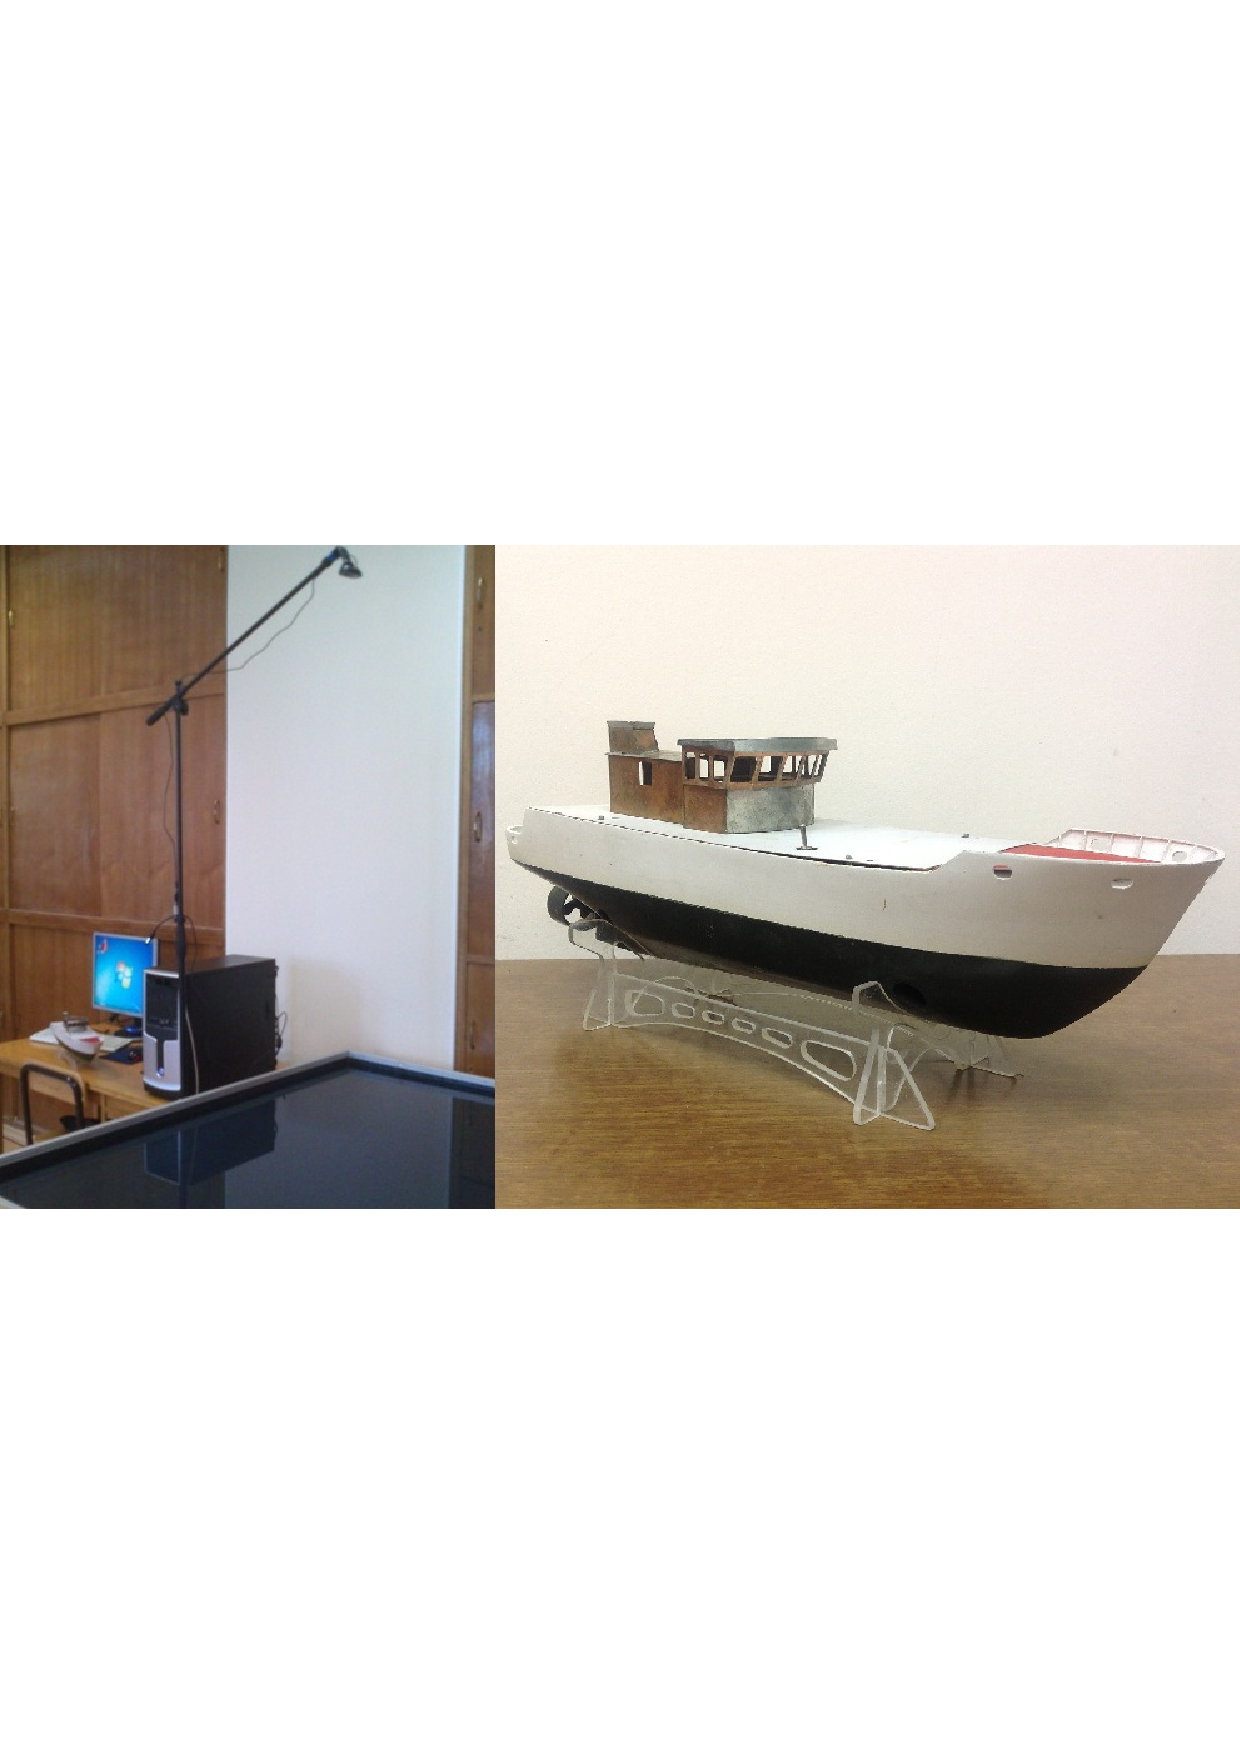
\includegraphics[width=9cm]{RBS.pdf}
\end{figure}

\centering
\qquad {Robotic Boat Setup}

\end{frame}

\begin{frame}{Robotic boat setup (RBS)}

\begin{columns}
\begin{column}{0.5\linewidth}
\begin{alertblock}{Type and size of the RBS} 
The robotic boat is a copy of the real trawler ship represented at a scale of 1:32. It's dimensions are $(0.432\times0.096\times0.052)\,m$
\end{alertblock}
The boat contains
\begin{itemize}
	\item the main engine
	\item two tunnel thrusters 
	\item servo drive for heading control
\end{itemize}
\end{column}
\begin{column}{0.5\linewidth}
	
\begin{figure}
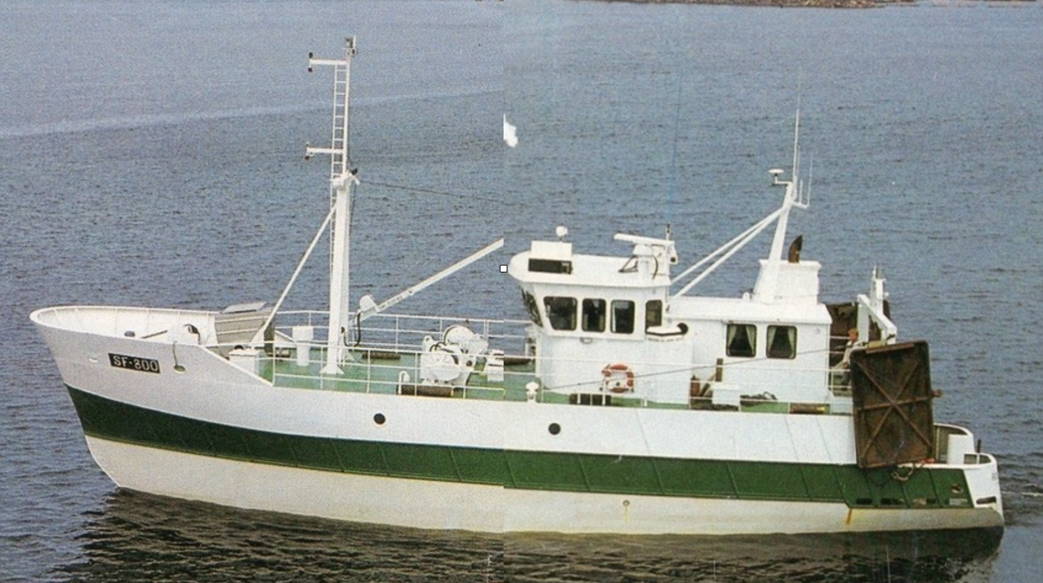
\includegraphics[width=4.5cm]{Rossvik.png}\quad
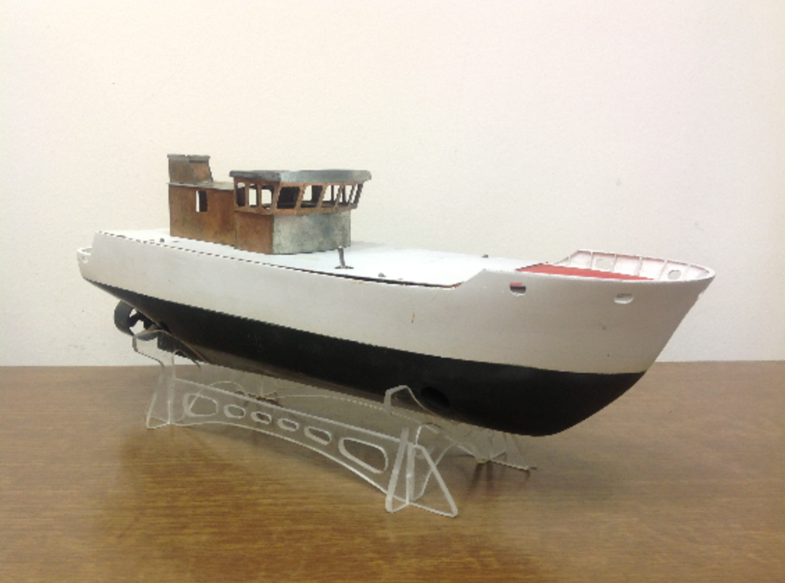
\includegraphics[width=4.5cm]{RBS_2.png}\quad
\end{figure}
 
 \centering
\qquad {Trawler "Rossvik" with a copy of a scale 1:32}

\end{column}
\end{columns}

\end{frame}

\section{Problem statement}

\begin{frame}

\begin{center}
	{\Large \textbf {Problem statement}\\}
\end{center}

Consider the linearised Nomoto's 2nd-order model, which represents behaviour of surface vessels

\begin{equation}
W(p)=\frac{K(1+T_3p)}{p(1+T_1p)(1+T_2p)},
\end{equation}

\begin{block}{Assumption 1}
Only the output variable is available for measurements. Its derivatives are unmeasurable.	
\end{block}

\begin{block}{Assumption 2}
	The polynomial $KT_3p+K$ is Hurwitz and $b_m=KT_3>0$. So, the model of the boat is minimum phase.	
\end{block}

\begin{block}{Assumption 3}
	The relative degree of the plant model $\rho=n-m=2$ is assumed to be known.
\end{block}

\end{frame}

\begin{frame}{Purpose}

The purpose of this paper is to design an output robust controller to the robotic boat in order to stabilize it in the specified position
\begin{eqnarray}
\lim_{t\rightarrow+\infty}x^*-x(t)&=&0\\
\lim_{t\rightarrow+\infty}y^*-y(t)&=&0\\
\lim_{t\rightarrow+\infty}\psi^*-\psi(t)&=&0
\end{eqnarray}

\begin{equation}
\label{u_sat}
\hat u(t)=\mathop{\mathrm{sat}}\nolimits u(t)=
\left\{
\begin{array}{ll}
u_{upp}, & \mbox{if $u(t)\ge u_{upp}$};\\
u(t), & \mbox{if $u_{low}<u(t)<u_{upp}$};\\
u_{low}, & \mbox{if $u(t)\le u_{low}.$}
\end{array}
\right.
\end{equation}

\vspace{0.2cm}
\centering where $u_{low}=-127$ and $u_{upp}=127$ 

\end{frame}

\section {Analysis of plant model}

\begin{frame}{Position and orientation of the boat}
	
%	\begin{center}
%		{\Large \textbf {Analysis of plant model}\\}
%	\end{center}
	
	Boat should be mathematically described by the MIMO model of the form
	\begin{eqnarray}
	\label{MIMO_model}
	x(t)&=&F(P_e, P_b, P_s, \alpha_e),\\
	y(t)&=&G(P_e, P_b, P_s, \alpha_e),\\
	\psi(t)&=&H(P_e, P_b, P_s, \alpha_e),
	\end{eqnarray}
	
	\begin{figure}
		\centering
		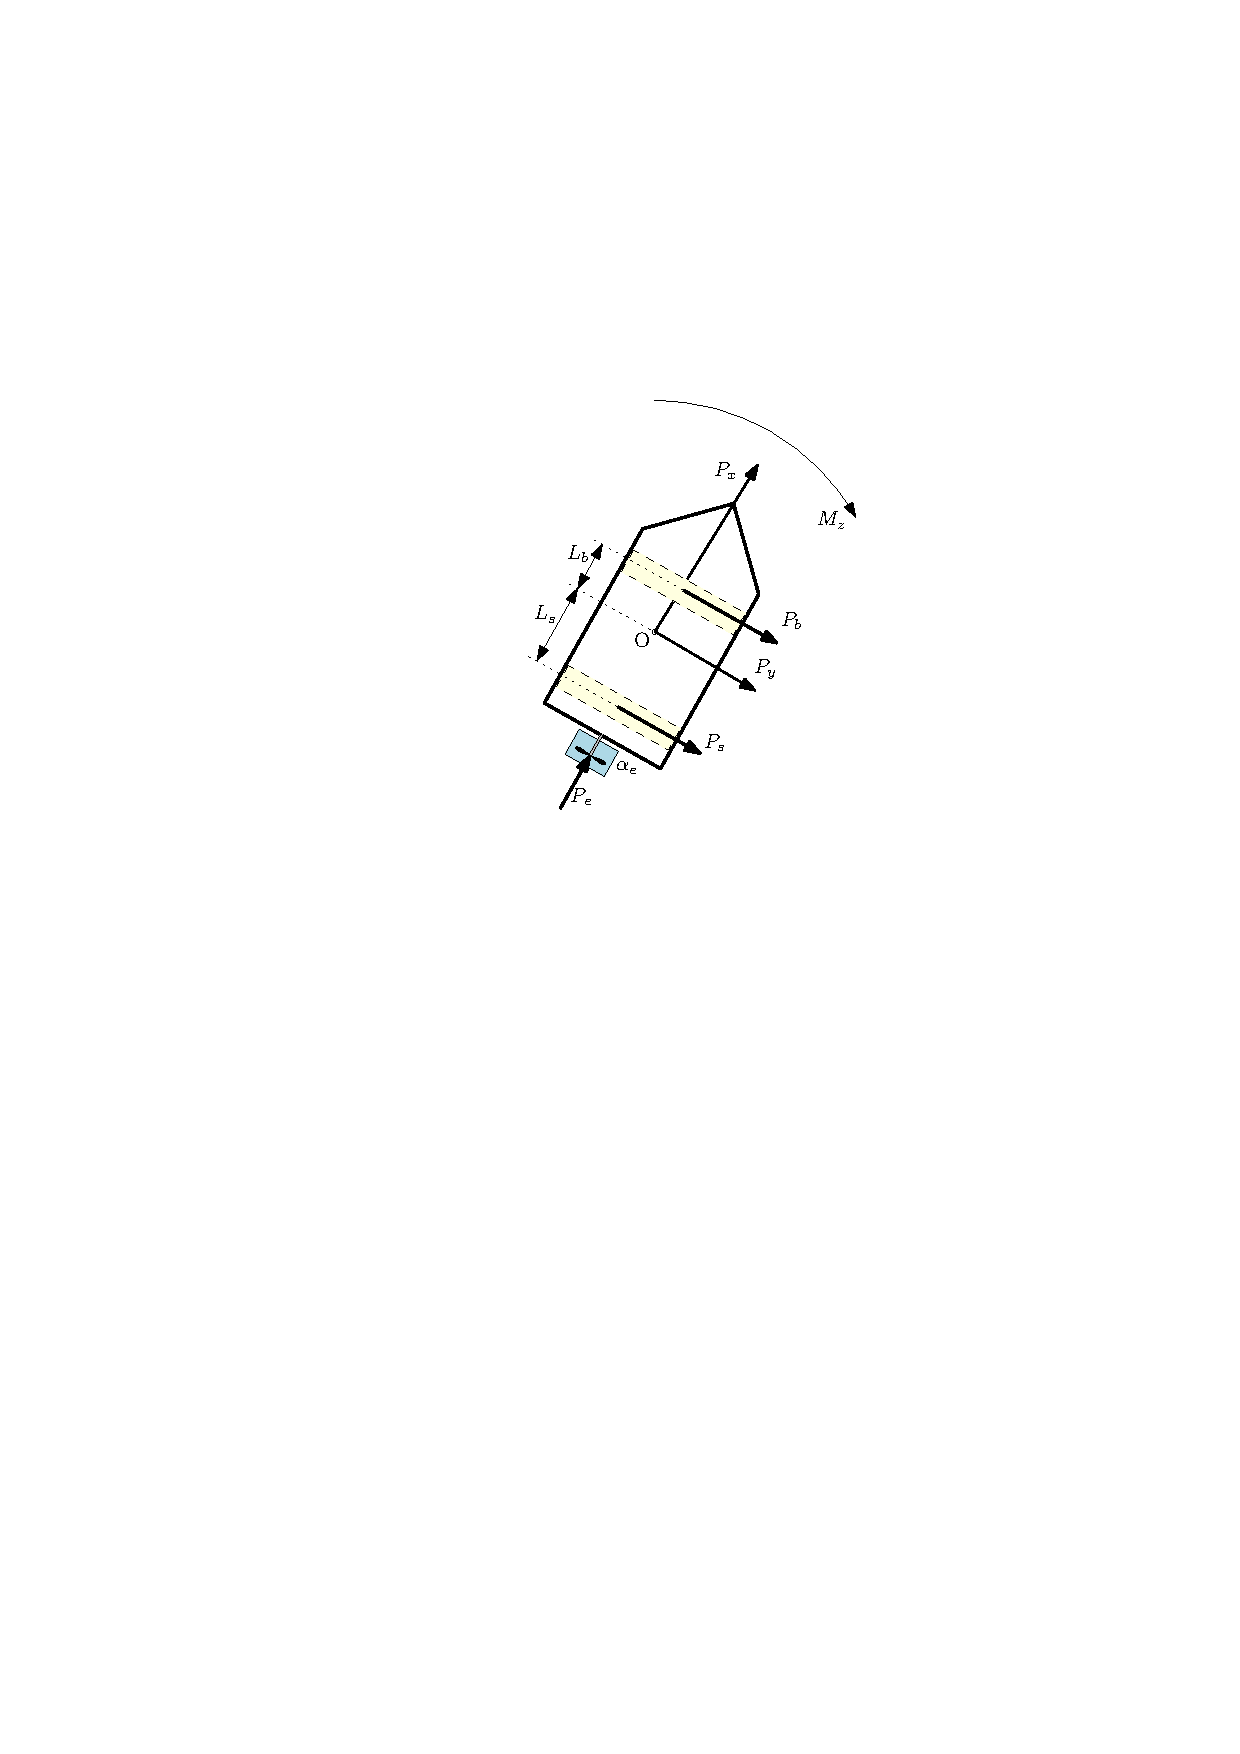
\includegraphics[height=4cm]{configuration}
		\caption{Generalized forces $P_x(t)$, $P_y(t)$ and moment $M_\psi(t)$}
	\end{figure}

\end{frame}


\begin{frame}{Decomposition}

To simplify control strategy perform decomposition of the model (\ref{MIMO_model}) as follows
\begin{eqnarray}
\label{decomposition}
&P_x(t)=P_e(t),&\\
&P_y(t)=P_b(t)+P_s(t),&\\
&M_\psi(t)=-\alpha_e(t)P_e(t)L_e+P_bL_b+P_sL_s,&
\end{eqnarray}


\end{frame}

\begin{frame}{Interconnections between the subsystems}

\begin{figure}[t]
	\centering
	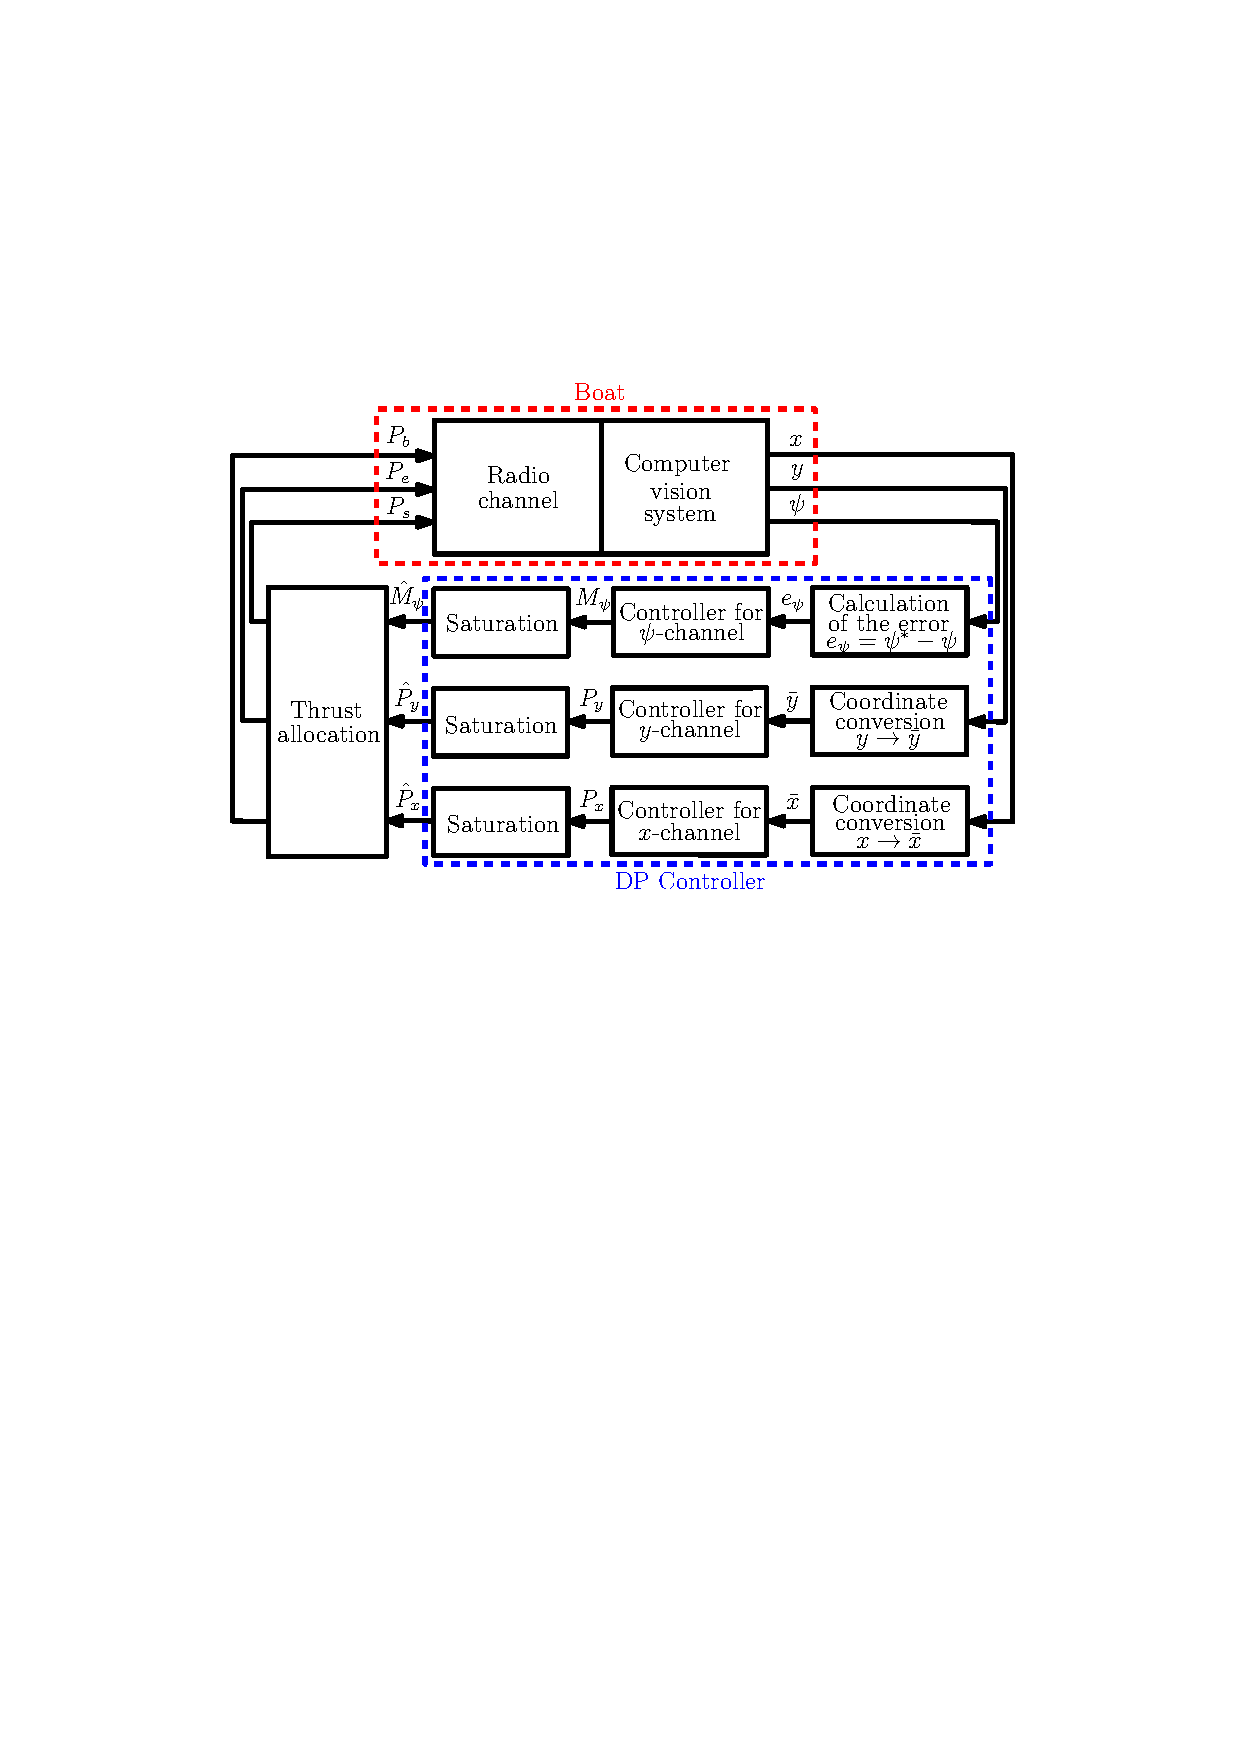
\includegraphics[width=8.4cm]{scheme}
	\caption{Interconnections between the subsystems}
	\label{scheme}
\end{figure}

\end{frame}

\begin{frame}{Computer vision}

The output variables of the computer vision system are the linear coordinates $x(t)$, $y(t)$ with respect to, say, the absolute coordinate system $(O,X,Y)$ and heading angle $\psi(t)$.

	\begin{figure}[b]
		\centering
		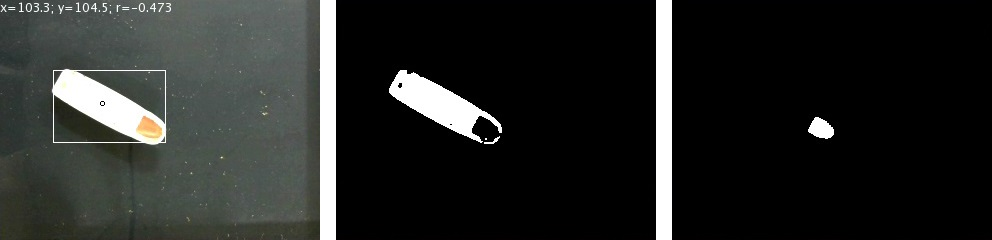
\includegraphics[width=11cm]{computer_vision}
		\caption{Visualization of the computer vision system}
		\label{computer_vision}
	\end{figure}

These signals are used to calculate the local coordinates $\bar x(t)$ and $\bar y(t)$ of the system $(\bar O,\bar X,\bar Y)$ attached to the boat and error $e_\psi(t)$ 

\end{frame}

\begin{frame}{Coordinate systems}

\begin{eqnarray}
&\begin{bmatrix}
	\bar x(t)\\
	\bar y(t)
\end{bmatrix}
=
\begin{bmatrix}
	\cos(\psi)&\sin(\psi)\\
	-\sin(\psi)&\cos(\psi)
\end{bmatrix}
\begin{bmatrix}
	x^*-x(t)\\
	y^*-y(t)
\end{bmatrix},&\\
&e_\psi=\psi^*-\psi(t),&
\end{eqnarray}

\begin{figure}[b]
	\centering
	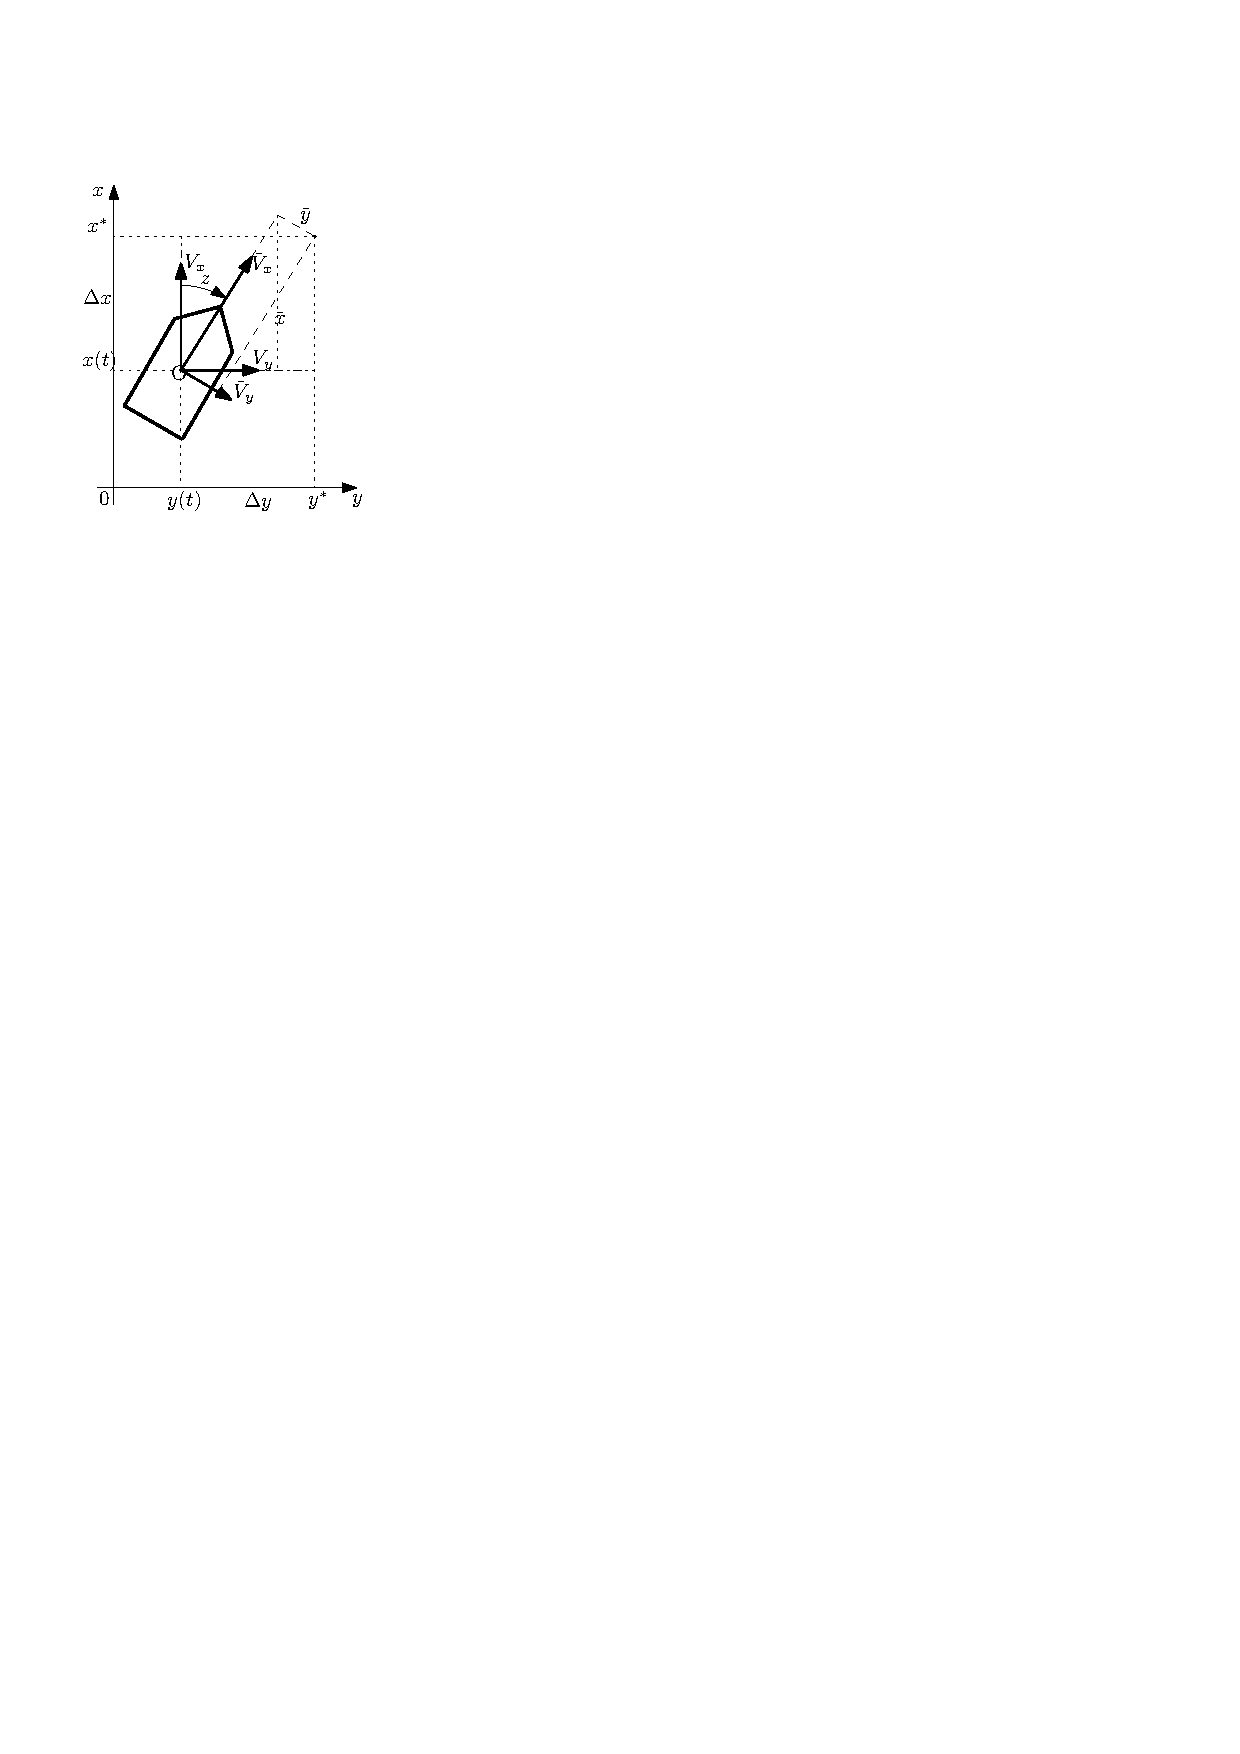
\includegraphics[height=5cm]{coordinate_systems}
	\caption{Coordinate systems $(O,X,Y)$ and $(\bar O,\bar X,\bar Y)$}
	\label{coordinate_systems}
\end{figure}

\end{frame}

\section {Control design}

\begin{frame}{Control design}

At the first step design a nominal linear controller under the assumption that the inputs are unbounded.

\begin{eqnarray}
\label{regular_control_law}
u(t)&=&\mu\alpha(p)\hat e(t),\\
\label{estimation_model_1}
\dot\xi(t)&=&\sigma(\Gamma\xi(t)+dk_1e(t))\\
\label{estimation_model_2}
\hat e(t)&=&h^T\xi(t),
\end{eqnarray}
where $\alpha(p)$ is the Hurwitz polynomial of the degree $(\rho-1)$, $\Gamma$, $d$, $h$ are matrices and vectors of corresponding dimensions

\begin{equation}
\Gamma=
\begin{bmatrix}
0 & 1 & 0 & \ldots & 0\\
0 & 0 & 1 & \ldots & 0\\
0 & 0 & 0 & \ldots & 0\\
\vdots & \vdots & \vdots & \ddots & \vdots\\
-k_1 & -k_2 & -k_3 & \ldots & -k_{\rho-1}
\end{bmatrix}\!,
d=
\begin{bmatrix}
0\\
0\\
0\\
\vdots\\
1
\end{bmatrix}\!,
h=
\begin{bmatrix}
1\\
0\\
0\\
\vdots\\
0
\end{bmatrix}\!,
\end{equation}
$k=\{k_1,k_2,\ldots,k_{\rho-1}\}$ are chosen for the estimation model (\ref{estimation_model_1}), (\ref{estimation_model_2}) to be stable.

\end{frame}

\begin{frame}{Control design}

As the polynomial $b(p)=K_iT_{3i}p+K_i$ is Hurwitz and $b_m=K_iT_{3i}>0$ all the imposed assumptions for this approach are satisfied. Apply the controller (\ref{regular_control_law}) with $\rho=2$, $\alpha(p)=p+1$ and write the controller explicitly
\begin{eqnarray}
&P_x=\mu_x(\dot\xi_x+\xi_x),\quad\dot\xi_x=\sigma_x(-\xi_x+\bar x),&\\
&P_y=\mu_y(\dot\xi_y+\xi_y),\quad\dot\xi_y=\sigma_y(-\xi_y+\bar y),&\\
&M_\psi=\mu_\psi(\dot\xi_\psi+\xi_\psi),\quad\dot\xi_\psi=\sigma_\psi(-\xi_\psi+e_\psi),&
\end{eqnarray} 
where $\mu_i$, $\sigma_i$, $i=\{x,y,\psi\}$ are the tuning coefficients, which can be chosen without knowledge of plant parameters.

\end{frame}

\begin{frame}{Realization of the scenario}
	
	\begin{figure}[t]
		\begin{center}
			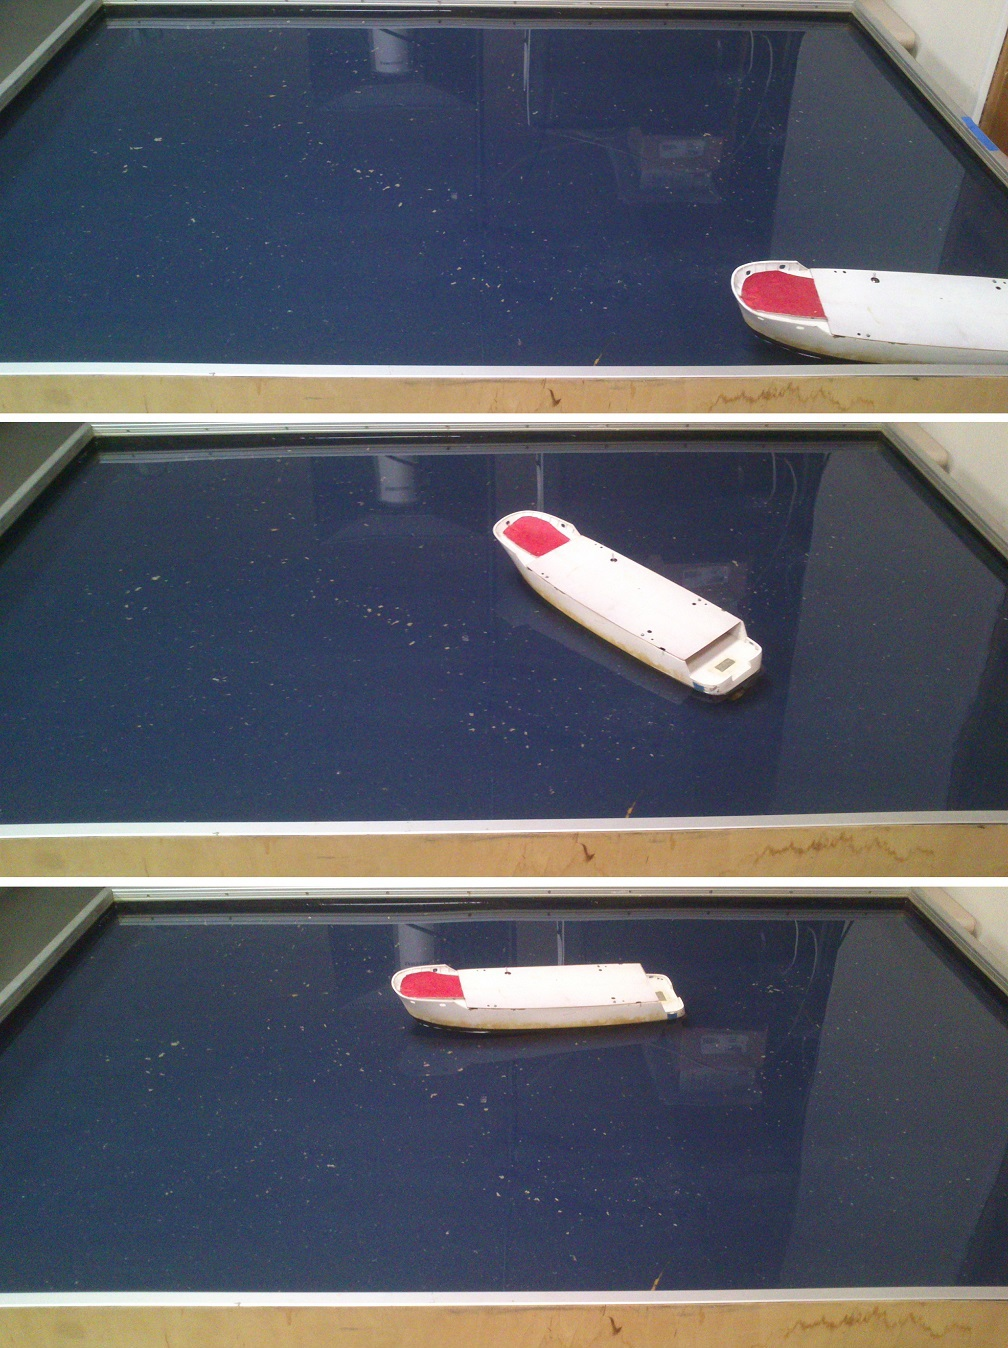
\includegraphics[width=5cm]{experiment}
			\caption{The boat goes to the specified point on the pool}
			\label{experiment}
		\end{center}
	\end{figure}

\end{frame}

\begin{frame}{Control design}

At the second step add an auxiliary integral loop by rewriting the control law (\ref{regular_control_law}) as follows
\begin{eqnarray}
\label{integral_control_law}
u(t)&=&\mu\frac{\beta(p)}{p}\hat e(t)=\mu\left(\gamma(p)+\frac{\beta_0}{p}\right)\hat e(t),\nonumber\\
&=&\mu\gamma(p)\hat e(t)-\mu\frac{\beta_0}{p}\hat e(t),
\end{eqnarray}
where $\gamma(p)$ is the part of the polynomial $\beta(p)$ excluding the free term $\beta_0$.

 At the third step according to this technique reconfigure the control law (\ref{integral_control_law}) by adding the mismatch signal between the saturated control and original one to the integral loop
 \begin{equation}
 \label{control_law_AW}
 u(t)=-\mu\gamma(p)\hat y(t)-\mu\frac{\beta_0}{p}(\hat y(t)+\psi(\hat u(t)-u(t))),
 \end{equation}
 where $\psi>0$ is some parameter.

\end{frame}

\begin{frame}{Control design}

The last step is allocating control among all the actuators. The virtual inputs should be transformed to the real ones. This may be carried out by the inverse transformation of (\ref{decomposition}). So, express the actuator inputs $P_e(t)$, $P_b(t)$ and $P_s(t)$ as follows
\begin{eqnarray}
&P_e(t)=P_x(t)&\\
&P_b(t)=P_y(t)-P_s(t)&\\
&P_s(t)=\frac{-\alpha_e(t) P_x(t)L_e+P_y(t)L_b-M_\psi}{L_b-L_s}.&
\end{eqnarray}

\end{frame}

\section{Experimental approval}

\begin{frame}

\begin{center}
	{\Large \textbf {Experimental approval}\\}
\end{center}

Construct three types of regulators in accordance to the previous section. The controller (\ref{regular_control_law}) is specified as
\begin{eqnarray}
\label{regular_control_law_experiment}
u(t)&=&-\mu\alpha(p)\hat y(t)=-0.5(1.5p+1)\hat y(t)\nonumber\\
&=&-0.5(1.5\dot{\hat y}(t)+\hat y(t)).
\end{eqnarray}

The controller augmented with the integral loop (\ref{integral_control_law}) has the form
\begin{eqnarray}
\label{integral_control_law_experiment}
u(t)&=&-\mu\frac{\beta(p)}{p}\hat y(t)=-0.5\frac{1.5p^2+p+0.05}{p}\hat y(t)\nonumber\\
&=&-0.5\left(1.5\dot{\hat y}(t)+\hat y(t)+0.05\int_0^t\hat y(\tau)d\tau\right).
\end{eqnarray}

\end{frame}

\begin{frame}{Controller with anti-windup scheme}

The next controller with the anti-windup scheme (\ref{control_law_AW}) is
\begin{eqnarray}
\label{control_law_AW_experiment}
u(t)&=&-\mu\gamma(p)\hat y(t)-\mu\frac{\beta_0}{p}(\hat y(t)+\psi(\hat u(t)-u(t)))\nonumber\\
&=&-0.5\left(1.5\dot{\hat y}(t)+\hat y(t)\right.\nonumber\\
&&\left.+0.05\int_0^t(\hat y(\tau)+4(\hat u(\tau)-u(\tau)))d\tau\right).
\end{eqnarray}

\begin{block}{Parameters of the experiment}
The input signal of the surface vessel model is constrained with the limits $-127\le\hat u(t)\le 127$ due to hardware design. The parameters of the estimation model (\ref{estimation_model_1}), (\ref{estimation_model_2}) are $\sigma=10$, $k_1=1$. In these experiments the dead zone of $\pm 2$ pixels ($\pm 0.006\mbox{ m}$) is specified in order to avoid switching of the control law in the neighbourhood of the equilibrium position (or the desired point). The dimensions of the boat are: length -- $0.432\mbox{ m}$, width -- $0.096\mbox{ m}$, height -- $0.052\mbox{ m}$. The dimensions of the pool are: length -- $1.60\mbox{ m}$, width -- $0.9\mbox{ m}$, depth -- $0.1\mbox{ m}$.
\end{block}

\end{frame}


\begin{frame}
	\frametitle{Experiment}
	\begin{figure}[ht]
		\setlength\fboxsep{0pt}
		\setlength\fboxrule{0.5pt}
		\fbox{
		
		}
		\label{fig:animation20}
	\end{figure}   
\end{frame}


\begin{frame}
	\frametitle{Experiment}
	\begin{figure}[ht]
		\setlength\fboxsep{0pt}
		\setlength\fboxrule{0.5pt}
		\fbox{
		
		}
		\label{fig:animation20}
	\end{figure}   
\end{frame}

\section{Results of the experiments}

\begin{frame}{Original and saturated control signals}

\begin{figure}[t]
	\begin{center}
		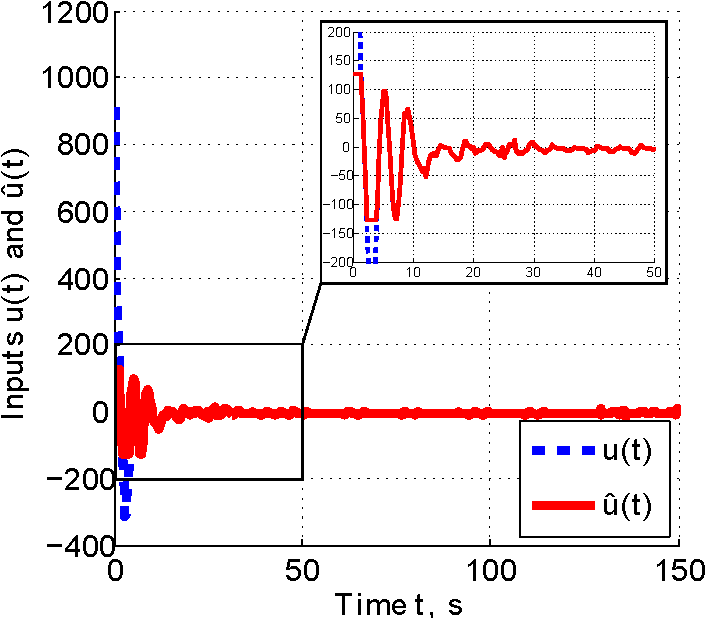
\includegraphics[height=6.5cm]{experimental_approval_inputs}
			\centering \caption{A plot of the original and saturated control signals generated by the consecutive compensator equipped with the anti-windup scheme tested on the robotic vessel complex}
		\label{experimental_approval_inputs}
	\end{center}
\end{figure}

\end{frame}

\begin{frame}
\begin{figure}[t]
	\begin{center}
		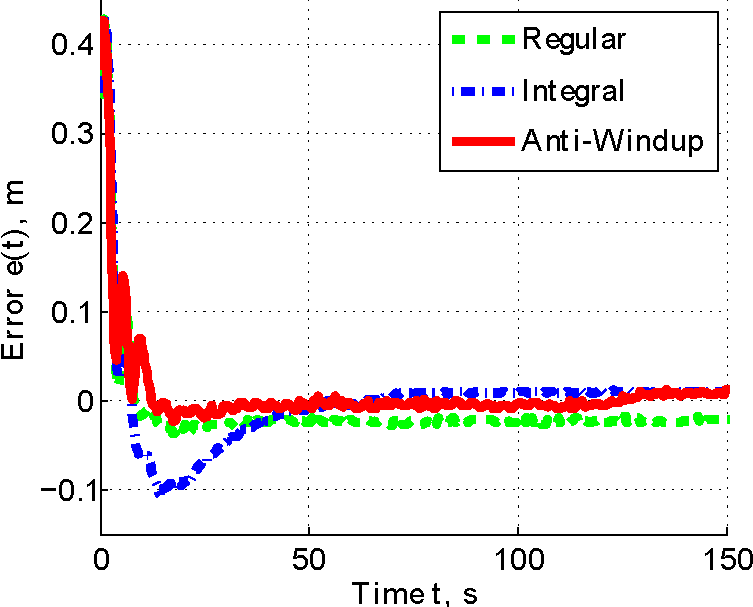
\includegraphics[height=6.5cm]{experimental_approval_error}
		\caption{Plots of the errors of the closed-loop system with various controllers tested on the robotic vessel complex}
		\label{experimental_approval_error}
	\end{center}
\end{figure}

\end{frame}

\section{Discussion}

\begin{frame}{Conclusion}

Development of simple control algorithms, which can be easily implemented to various real technical systems with bounded inputs presented in this practical study.

\begin{itemize}
	\item The result of this work can be useful in stabilization tasks of various applications 
	\item The proposed controller has shown the satisfactory experimental results at the robotic boat setup  
	\item This approach is applicable for plants with bounded input and uncertain parameters  
\end{itemize}
\end{frame}

\begin{frame}
	\begin{center}
		{\huge Thank you for your attention!}
	\end{center}
	\vspace{\baselineskip}
	\begin{center}
		Contact information
	\end{center}
	\begin{center}
		\begin{columns}
			\column{0.5\textwidth}
			Igor Petranevsky\\
			igor.petranevsky@corp.ifmo.ru \\
			\vspace{\baselineskip}
			Anton Pyrkin\\
			pyrkin@corp.ifmo.ru
			\column{0.5\textwidth}
			\begin{center}
				
\includegraphics[width = 50mm]{fig/itmo1.png}
			\end{center}
		\end{columns}
	\end{center}
\end{frame}

\end{document}